\documentclass[
letterpaper,
11pt,
%answers,
]{exam}

\usepackage[lmargin=0.75in,rmargin=0.75in,tmargin=1in,bmargin=1in]{geometry}
\usepackage{soul}
\usepackage{enumitem}
\usepackage{graphicx}
\usepackage{tikz}
\usepackage{multicol}
\usepackage[randomize]{exam-randomizechoices}
\setrandomizerseed{28056}

% Sets the column separation so that enumeration doesn't cause
% the line between columns interfere with the numbers.
\setlength{\columnsep}{4em}
\setlength{\columnseprule}{0.4pt}

% If multicolumn, it reduces the indentation of the multiple choice answers.
%\renewcommand{\choiceshook}{\setlength{\leftmargin}{20pt}}

% Code block creates the Matching question format
\newcommand*\Matching[1]{
\ifprintanswers
\textbf{#1}
\else
\rule{1in}{0.5pt}
\fi
}
\newlength\matchlena
\newlength\matchlenb
\settowidth\matchlena{\rule{1in}{0pt}}
\newcommand\MatchQuestion[2]{%
\setlength\matchlenb{\linewidth}
\addtolength\matchlenb{-\matchlena}
\parbox[t]{\matchlena}{\Matching{#1}}\enspace\parbox[t]{\matchlenb}{#2}}

% Formats the header on the first page where the student enters their name and date.
\newcommand{\head}{%
\thispagestyle{empty}
\vspace*{-0.75in}
\noindent
\class \hfill Name \makebox[7cm]{\hrulefill} Ver: \wsVer\par
\vspace{10pt}
\noindent
\Large\textbf{\wstitle}\normalsize \hfill Date \makebox[3.5cm]{\hrulefill}\par
\vspace{10pt}
\noindent
\textit{\Instructions}
}

% Defines the titles and instructions for the worksheet or test
\newcommand{\class}{Humanities}
\newcommand{\wstitle}{\textit{Template} Test}
\newcommand{\wsVer}{1}
\newcommand{\Instructions}{}

% Sets the running header at the top of the subsequent pages
\pagestyle{head}
\runningheader{\class\ \wstitle}{}{Page \thepage\ of \numpages}

% BEGINNING OF DOCUMENT
\begin{document}
\head
\setlength{\linewidth}{6.5in}

% Moves the first heading up a smidge. The space before it was too big.
\vspace{-0.4in}


% Begin copy-and-pasting your sections here.
% Copy  this whole column for a section of matching questions.
\section*{Geography Matching}
%\vspace{-1\baselineskip}
%\fullwidth{%

\begin{tikzpicture}
    % Include the image
    \node[anchor=south west,inner sep=0] at (0,0) {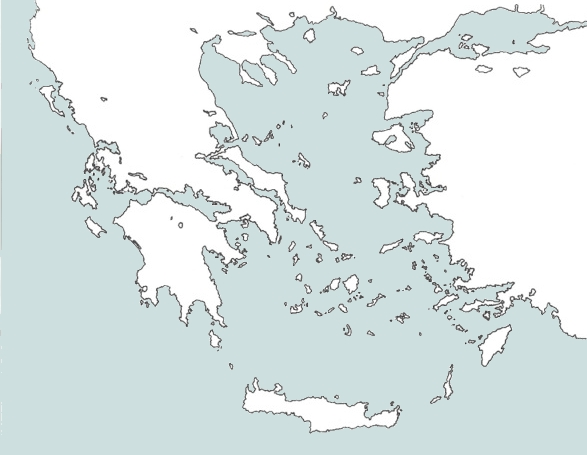
\includegraphics[width=\textwidth]{blankGreekmap.jpg}};

    % Overlay text at specific coordinates
    \node at (1, 1) {\small 1,1};  % Adjust coordinates and text size
    \node at (2, 2) {\small 2,2};
    \node at (3, 3) {\small 3,3};
    \node at (4, 4) {\small 4,4};
    \node at (5, 5) {\small 5,5};
    \node at (6, 6) {\small 6,6};
    \node at (7, 7) {\small 7,7};
    \node at (8, 8) {\small 8,8};
    \node at (9, 9) {\small 9,9};
    \node at (10, 1.2) {\small Crete};
    \node at (11, 11) {\small 11,11};
    \node at (12, 12) {\small 12,12};
    \node at (13, 13) {\small 13,13};
    \node at (14, 14) {\small 14,14};
    \node at (15, 14) {\small 15,14};
    \node at (16, 14) {\small 16,14};
    \node at (17, 14) {\small 16,14};
\end{tikzpicture}
%}

\textit{Fill in each blank with the appropriate letter.}\par

\begin{questions}

\begin{multicols}{2}
\question\MatchQuestion{A}{rhinoceros} \vfill
\question\MatchQuestion{Boeotia}{Boeotia} \vfill
\question\MatchQuestion{Mycenaia}{Mycenaia} \vfill
\question\MatchQuestion{Troy}{Troy} \vfill
\question\MatchQuestion{Olympia}{Olympia} \vfill
\question\MatchQuestion{Corinth}{Corinth} \vfill
\question\MatchQuestion{Sparta}{Sparta} \vfill
\end{multicols}

\end{questions}
\end{document}